% Search for all the places that say "PUT SOMETHING HERE".

\documentclass[11pt]{article}
\usepackage{amsmath,textcomp,amssymb,geometry,graphicx,enumerate}

\def\Name{Ran Liao}  % Your name
\def\SID{3034504227}  % Your student ID number
\def\Homework{8} % Number of Homework
\def\Session{Spring 2019}


\title{CS170--Spring 2019 --- Homework \Homework\ Solutions}
\author{\Name, SID \SID}
\markboth{CS170--\Session\  Homework \Homework\ \Name}{CS170--\Session\ Homework \Homework\ \Name}
\pagestyle{myheadings}
\date{\today}

\newenvironment{qparts}{\begin{enumerate}[{(}a{)}]}{\end{enumerate}}
\def\endproofmark{$\Box$}
\newenvironment{proof}{\par{\bf Proof}:}{\endproofmark\smallskip}

\textheight=9in
\textwidth=6.5in
\topmargin=-.75in
\oddsidemargin=0.25in
\evensidemargin=0.25in


\begin{document}
\maketitle
Collaborators:Jingyi Xu, Renee Pu

\section{Study Group}
	\begin{tabular}{ll}
		Name		&   SID         		\\\hline
		Ran Liao		&   3034504227  	\\  
		Jingyi Xu		&   3032003885  	\\
		Renee Pu		&   3032083302  	\\
	\end{tabular}

	



\newpage
\section{Modeling: Tricks of the Trade}
\begin{qparts}
	
	\item 
	
	\[
		\min z_1 + z_2 + \cdots + z_n
	\]
	\[
		z_i \ge y_i - (a + bx_i)  \text{ for } i = 1, \cdots, n
	\]
	\[
		z_i \ge -(y_i - (a + bx_i))  \text{ for } i = 1, \cdots, n
	\]
	
	\item 
	
	\[
		\min z
	\]
	\[
		z \ge y_i - (a + bx_i)  \text{ for } i = 1, \cdots, n
	\]
	\[
		z \ge -(y_i - (a + bx_i))  \text{ for } i = 1, \cdots, n
	\]
		
\end{qparts}



\newpage
\section{Zero Sum Games}
\begin{qparts}
	\item 
	
	$x_1$ is the probability that Alice will play strategy $1$. 
	
	$x_2$ is the probability that Alice will play strategy $2$.
	
	$p$ is an artificial variable.
	
	\item
	
	\[
		\max p
	\]
	\[
		p \le 4x_1 +2x_2
	\]
	\[
		p \le x_1 +5x_2
	\]
	\[
		x_1 + x_2 = 1
	\]
	\[
		x_1 \ge 0
	\]
	\[
		x_2 \ge 0
	\]

	\item
	
	\[
		\max p
	\]
	\[
		p \le 4x_1 +2(1 - x_1) = 2x_1 + 2
	\]
	\[
		p \le x_1 +5(1 - x_1) = -4x_1 + 5
	\]
	\[
		0 \le x_1 \le 1
	\]
	
	\item \text{ }
	
	\begin{figure}[h]
	\centering
	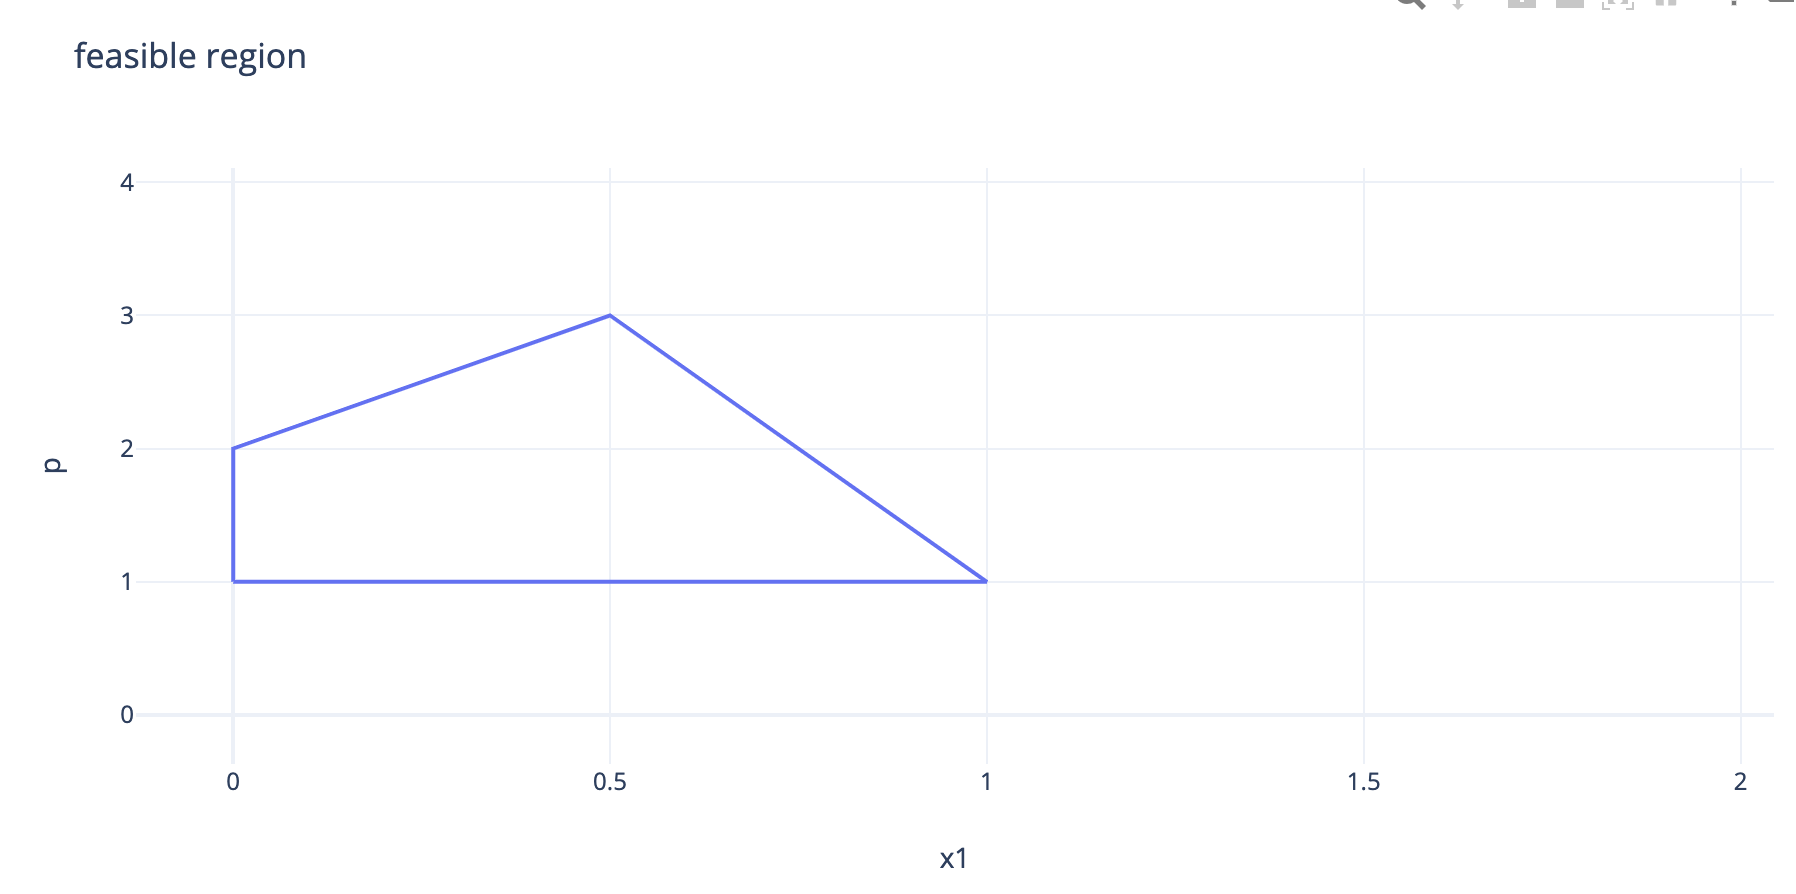
\includegraphics[width=.8\textwidth]{feasible_region.png}
	\caption{\label{fig:feasible_region}Feasible Region}
	\end{figure}
	
	\item
	
\end{qparts}




\newpage
\section{Triangulating a polygon}
\begin{qparts}
	\item \textbf{Main Idea}
	
	First sort all points into clockwise order and denote $D[i][j]$ as the distance between $i$th point and $j$th point, i.g. $D[i][j] = \sqrt{(x_i - x_j)^2 + (y_i - y_j)^2}$.
	
	Define subproblem as $T[i][j]$, which represents the optimal solution to triangulate polygon defined by $i$th point to $j$th point.
	The recursive relation is as follows. In base case, if $j - i < 3$, $T[i][j]$ is 0.
	\[
		T[i][j] = \min \{ \min_{k=i+2}^{j-2}\{ T[i][k] + T[k][j] + D[i][k] + D[j][k] \}, T[i][j-1] + D[i][j-1], T[i+1][j], + D[i+1][j]\}    
	\]
	
	
	 And the final solution is $T[1][n]$.

	\item \textbf{Proof of Correctness}
	
	In base case, triangle do not need to be triangulated, so the cost is 0. In induction step, for $T[i][j]$, we have $j - i - 1$ ways to choose an vertex $k$, so that breaks it into two or one subproblems. One subproblem is triangulate polygon defined by $i$th point to $k$th point. The other is triangulate polygon defined by $k$th point to $j$th point. Choose the smallest cost among them can guarantee the optimality of $T[i][j]$. Therefore the final answer $T[1][n]$ is optimal. 
	
	\item \textbf{Runtime Analysis}
	
	There're $n^2$ subproblems and each of them will cost $O(n)$ time to check each possible situation. Therefore, the overall runtime is $O(n^3)$.

\end{qparts}

\newpage
\section{Three Partition}
\begin{qparts}
	\item \textbf{Main Idea}
	
	Define subproblem as $X[i][s_1][s_2]$, which represents whether it's possible to divide first $i$ numbers into three groups, such that the sum of first group is $s_1$ and the sum of second group is $s_2$. Suppose the $i$th number is $A[i]$.
	The recursive relation is as follows:
	\[
		X[i][s_1][s_2] = X[i-1][s_1][s_2] \lor X[i-1][s_1 - A[i]][s_2] \lor X[i-1][s_1][s_2 - A[i]]
	\]
	
	 And the final solution is $X[n][\frac{total}{3}][\frac{total}{3}]$.

	\item \textbf{Proof of Correctness}
	
	In base case, $X[1][0][0]$, $X[1][A[1]][0]$ and $X[1][0][A[1]]$ are true. This is trivial. In induction step, for $X[i][s_1][s_2]$ we have three choices, i.g. put $i$th number into first group, second group or third group. $X[i-1][s_1][s_2]$ is the situation that put it into first group. $X[i-1][s_1 - A[i]][s_2]$ is the situation that put it into second group. $X[i-1][s_1][s_2 - A[i]]$ is the situation that put it into third group. So $X[i][s_1][s_2]$ will be optimal and the final answer will be optimal.
	
	\item \textbf{Runtime Analysis}
	
	There're $n(\sum a_i)^2$ subproblems and each of them will cost $O(1)$ time. Therefore, the overall runtime is $O(n(\sum a_i)^2)$.	

\end{qparts}

\newpage
\section{2-SAT}
\begin{qparts}
	
	\item 

	if $G_I$ has a strongly connected component containing both $x$ and $\neg x$ for some variable $x$. Then there's a path from $x$ to $\neg x$ and a path from $\neg x$ to $x$. The edges in this graph can be considered as implication, so we have $x \Rightarrow  \neg x$ and $\neg x \Rightarrow  x$ by transitive rule.
	So if $x$ is assigned with true, we have contradiction $true\Rightarrow false$. If  $x$ is assigned with false, we have $true\Rightarrow false$ as well. Therefore this problem has no valid solution.
	
	\item
	
	Note that the clause $(\alpha \lor \beta)$ is equivalent to $(\neg \alpha  \Rightarrow \beta) \land (\neg \beta\Rightarrow  \alpha)$. The edges added in to graph $G_I$ is symmetric. 
	
	Suppose SCC $A$ contains variables $v_1, v_2, v_3, \cdots v_n$. By symmetric property, there exists SCC $\neg A$ that contains variables $\neg v_1, \neg v_2, \neg v_3, \cdots \neg v_n$. Similarly, if there's an edge from SCC $A$ to SCC $B$, there exist an edge from SCC $\neg B$ to $\neg A$.
	
	In base case, there're only two SCCs and denote them as $A$ and $\neg A$. This is trivial. Assigned one of them with true and the other with false will satisfy requirement. In induction step, suppose SCC $A$ is a sink. Then SCC $\neg A$ must be a source. Suppose there's an edge from SCC $B$ to SCC $A$. Then there's an edge from SCC $\neg A$ to SCC $\neg B$. Assign $A$ with all trues can guarantee edge from SCC $B$ to SCC $A$ is satisfied. And assign $\neg A$ with all false can guarantee edge from SCC $\neg A$ to SCC $\neg B$ is satisfied. Therefore, delete all of them will not introduce conflicts and can always find a satisfaction solution.
	
	\item
	
	So first compute SCCs (meta-graph $G_M$ of $G_I$) and assign value according to the previous mentioned way. Compute meta graph will cost $(O(|E| + |V|))$ time and assign will cost linear time. So the total runtime is linear.
		
\end{qparts}






\end{document}